\section*{Problem 4 LTI convolution}
Let 
\begin{align}
    h[n] = 2(u[n] - u[n-5]),
\end{align}

be an impulse response of some system and 
\begin{align}
    x[n] = u[n] - u[n-3]
\end{align}

the input.
\subsection*{Discrete case}
\subsubsection*{Scetch both}
\begin{lstlisting}[language=python]
# imports
import numpy as np
import matplotlib.pyplot as plt


# define series
def h_fn(n):
    return 2*(np.heaviside(n, 1) - np.heaviside(n-5, 1))

def x_fn(n):
    return np.heaviside(n, 1) - np.heaviside(n-3, 1)

# define ns
ns = np.arange(-3,10)


#plot 
fig, ax = plt.subplots()
ax.stem(ns, h_fn(ns), linefmt='tab:blue', label='h[n]')
ax.stem(ns, x_fn(ns), linefmt='tab:orange', label='x{n]')

ax.legend()
plt.savefig("figures/p4_stems.png")
plt.show()
\end{lstlisting}
\clearpage

\begin{figure}[h!]
    \begin{center}
        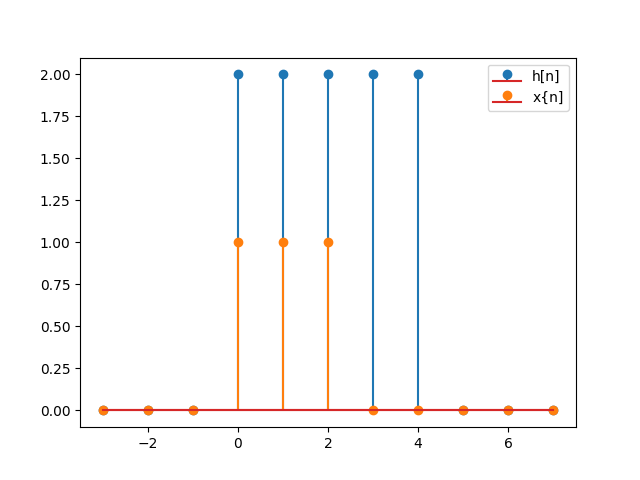
\includegraphics[width=0.95\textwidth]{figures/p4_stems.png}
    \end{center}
    \caption{Input and impulse response.}
\end{figure}

\subsubsection*{Sketch the convolution}
\begin{lstlisting}[language=python]
ys = np.convolve(xs, hs)
ks = np.arange(-(n + n), m + m - 1)

#plot 
fig, ax = plt.subplots()
ax.stem(ks, ys, linefmt='tab:green', label='y[n]')
ax.set_xlim([-3, 10])
ax.legend()
plt.savefig("figures/p4_conv.png")
plt.show()
\end{lstlisting}
\clearpage

\begin{figure}[h!]
    \begin{center}
        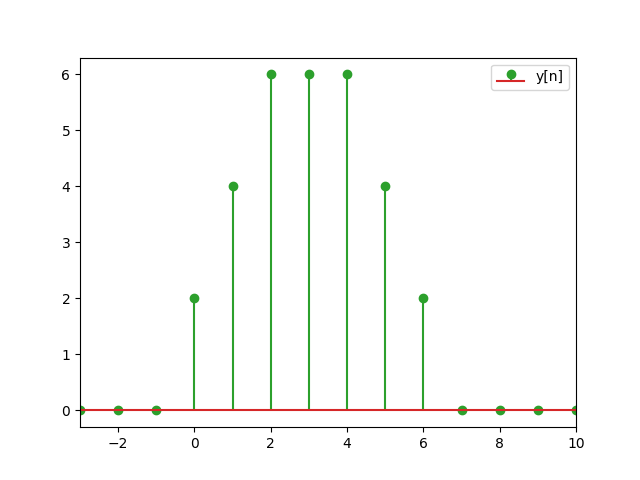
\includegraphics[width=0.95\textwidth]{figures/p4_conv.png}
    \end{center}
    \caption{Output.}
\end{figure}

\subsection*{Continuous case}
Let 
\begin{align}
    h(t) = (u(t) - u(t)),
\end{align}

be an impulse response of some system and 
\begin{align}
    x(t) = u(t) - u(t-3)
\end{align}

the input.
\subsubsection*{Scetch both}
\begin{lstlisting}[language=python]
# imports
import numpy as np
import matplotlib.pyplot as plt


# define series
def h_fn(t):
    return np.heaviside(t, 1) - np.heaviside(t-5, 1)

def x_fn(t):
    return np.heaviside(t, 1) - np.heaviside(t-3, 1)

# define ns
n, m = 3, 8
ts = np.linspace(-n, m, 100)
xs, hs = x_fn(ts), h_fn(ts)

#plot 
fig, ax = plt.subplots()
ax.plot(ts, hs, label='h[n]')
ax.plot(ts, xs, label='x{n]')

ax.legend()
plt.savefig("figures/p4_stems_ct.png")
plt.show()
\end{lstlisting}
\clearpage

\begin{figure}[h!]
    \begin{center}
        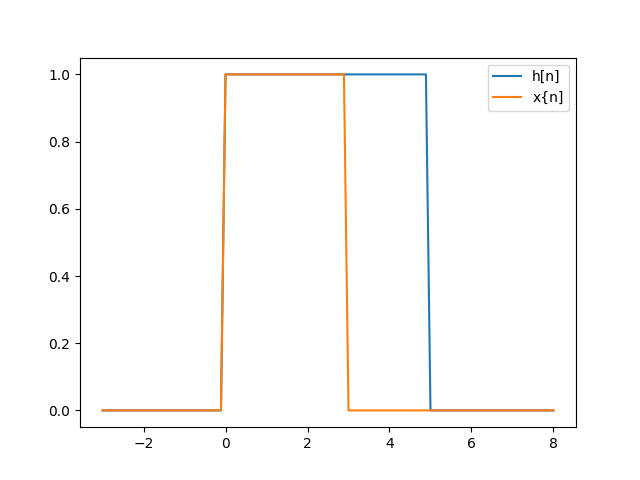
\includegraphics[width=0.95\textwidth]{figures/p4_stems_ct.png}
    \end{center}
    \caption{Input and impulse response.}
\end{figure}

\subsection*{Sketch convolution}
We find this by integration
\begin{align}
    y(t)    &= h(t)*x(t)\\ 
            &= \int_\mathbb{R}d\lambda \ \ h(\lambda)x(t-\lambda)\\
            &= \int_\mathbb{R}d\lambda \ \ (u(\lambda) - u(\lambda-5))
                (u(t-\lambda) - u(t-\lambda-3))\\
            &= \int_0^5d\lambda \ \ u(t-\lambda) - u(t-\lambda-3)\\ 
            &= \int_0^5 d\lambda \ \ u(t-\lambda) 
                - \int_0^5 d\lambda \ \ u(t - \lambda - 3).
\end{align}

Then 
\begin{align}
    y(t) &= \begin{cases}
    0, &\text{ if }t<0\\
    \int_0^t d\lambda = t, &\text{ if }0\leq t<3\\
        \int_0^t d\lambda  - \int_0^{t-3} d\lambda 
            \ \ = 3, &\text{ if }3\leq t<5\\
        \int_0^5 d\lambda  - \int_0^{t -3} d\lambda \ \ 
            = 8 - t, &\text{ if }t\leq 8\\
    0, &\text{ if }t >8\\
\end{cases}
\end{align}


\begin{lstlisting}[language=python]
def ys_fn(t):
    out = np.zeros_like(t)
    out[t < 8] = 8. -t[t<8]
    out[t < 5] = 3.
    out[t < 3] = t[t<3]
    out[t<0] = 0.

    return out

ts = np.linspace(-(n + n), m + m - 1, 100)
ys = ys_fn(ts)

#plot 
fig, ax = plt.subplots()
ax.plot(ts, ys, 'tab:green', label='y[n]')
ax.set_xlim([-3, 10])
ax.legend()
plt.savefig("figures/p4_conv_ct.png")
plt.show()
\end{lstlisting}

\clearpage

\begin{figure}[h!]
    \begin{center}
        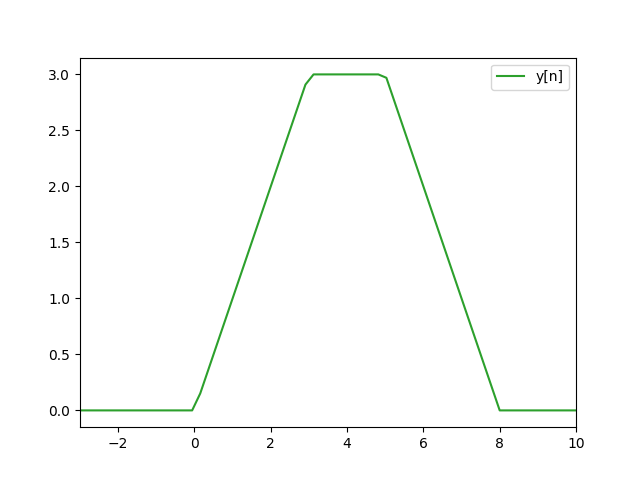
\includegraphics[width=0.95\textwidth]{figures/p4_conv_ct.png}
    \end{center}
    \caption{Output.}
\end{figure}

Unsurpirisngly this looks alot like the d.t. case.

